\fancyhead[L]{Chapter I}
\fancyhead[R]{General project context}

\vspace*{9cm}
\begin{doublespace}
    \centering
    \addcontentsline{toc}{chapter}{Chapter I: Work context}
    \textbf{ \huge Chapter I \\ [1 cm] General project context}
\end{doublespace} 

\newpage
\fancyhead[R]{\rightmark}

\doublespacing

\section*{Introduction}

This chapter presents the general context of the project, beginning with an overview of Renault Group and its Moroccan subsidiary, Renault Digital Morocco. It then introduces the Key Management System (KMS) project and the specific challenges related to cryptographic resource lifecycle management. Finally, it outlines the project objectives, management methodology, and planning approach used throughout the development process.

\section{Presentation of Renault}

\subsection{Renault Group}
The \textbf{Renault Group} is a major French company that designs and manufactures cars and commercial vehicles, with a history dating back to 1899. Today, it operates globally and brings together well-known brands such as Renault, Dacia, Alpine and Mobilize. \\

\noindent
The \textbf{Renault Group} was founded in 1899 by Louis Renault and his brothers, and quickly became known for its spirit of innovation and ability to mass produce in the automotive industry. The company played an important role during both world wars, was nationalized in 1945, then privatized in 1996. In 1999, Renault formed a strategic alliance with Nissan and expanded internationally by acquiring brands such as Dacia and Samsung Motors, with a desire to strengthen itself in global markets and modernize its operations.


\subsection{Renault Group Morocco}
\textbf{Renault Group Morocco} is a key player in the automotive industry in Morocco, with two major production sites: the SOMACA plant in Casablanca and the Tangier plant.
In addition to these two production sites, Renault Group Morocco relies on a well-integrated ecosystem composed of five key entities, each playing an essential role in the group's success, both locally and internationally.


\begin{figure}[H]
    \centering
    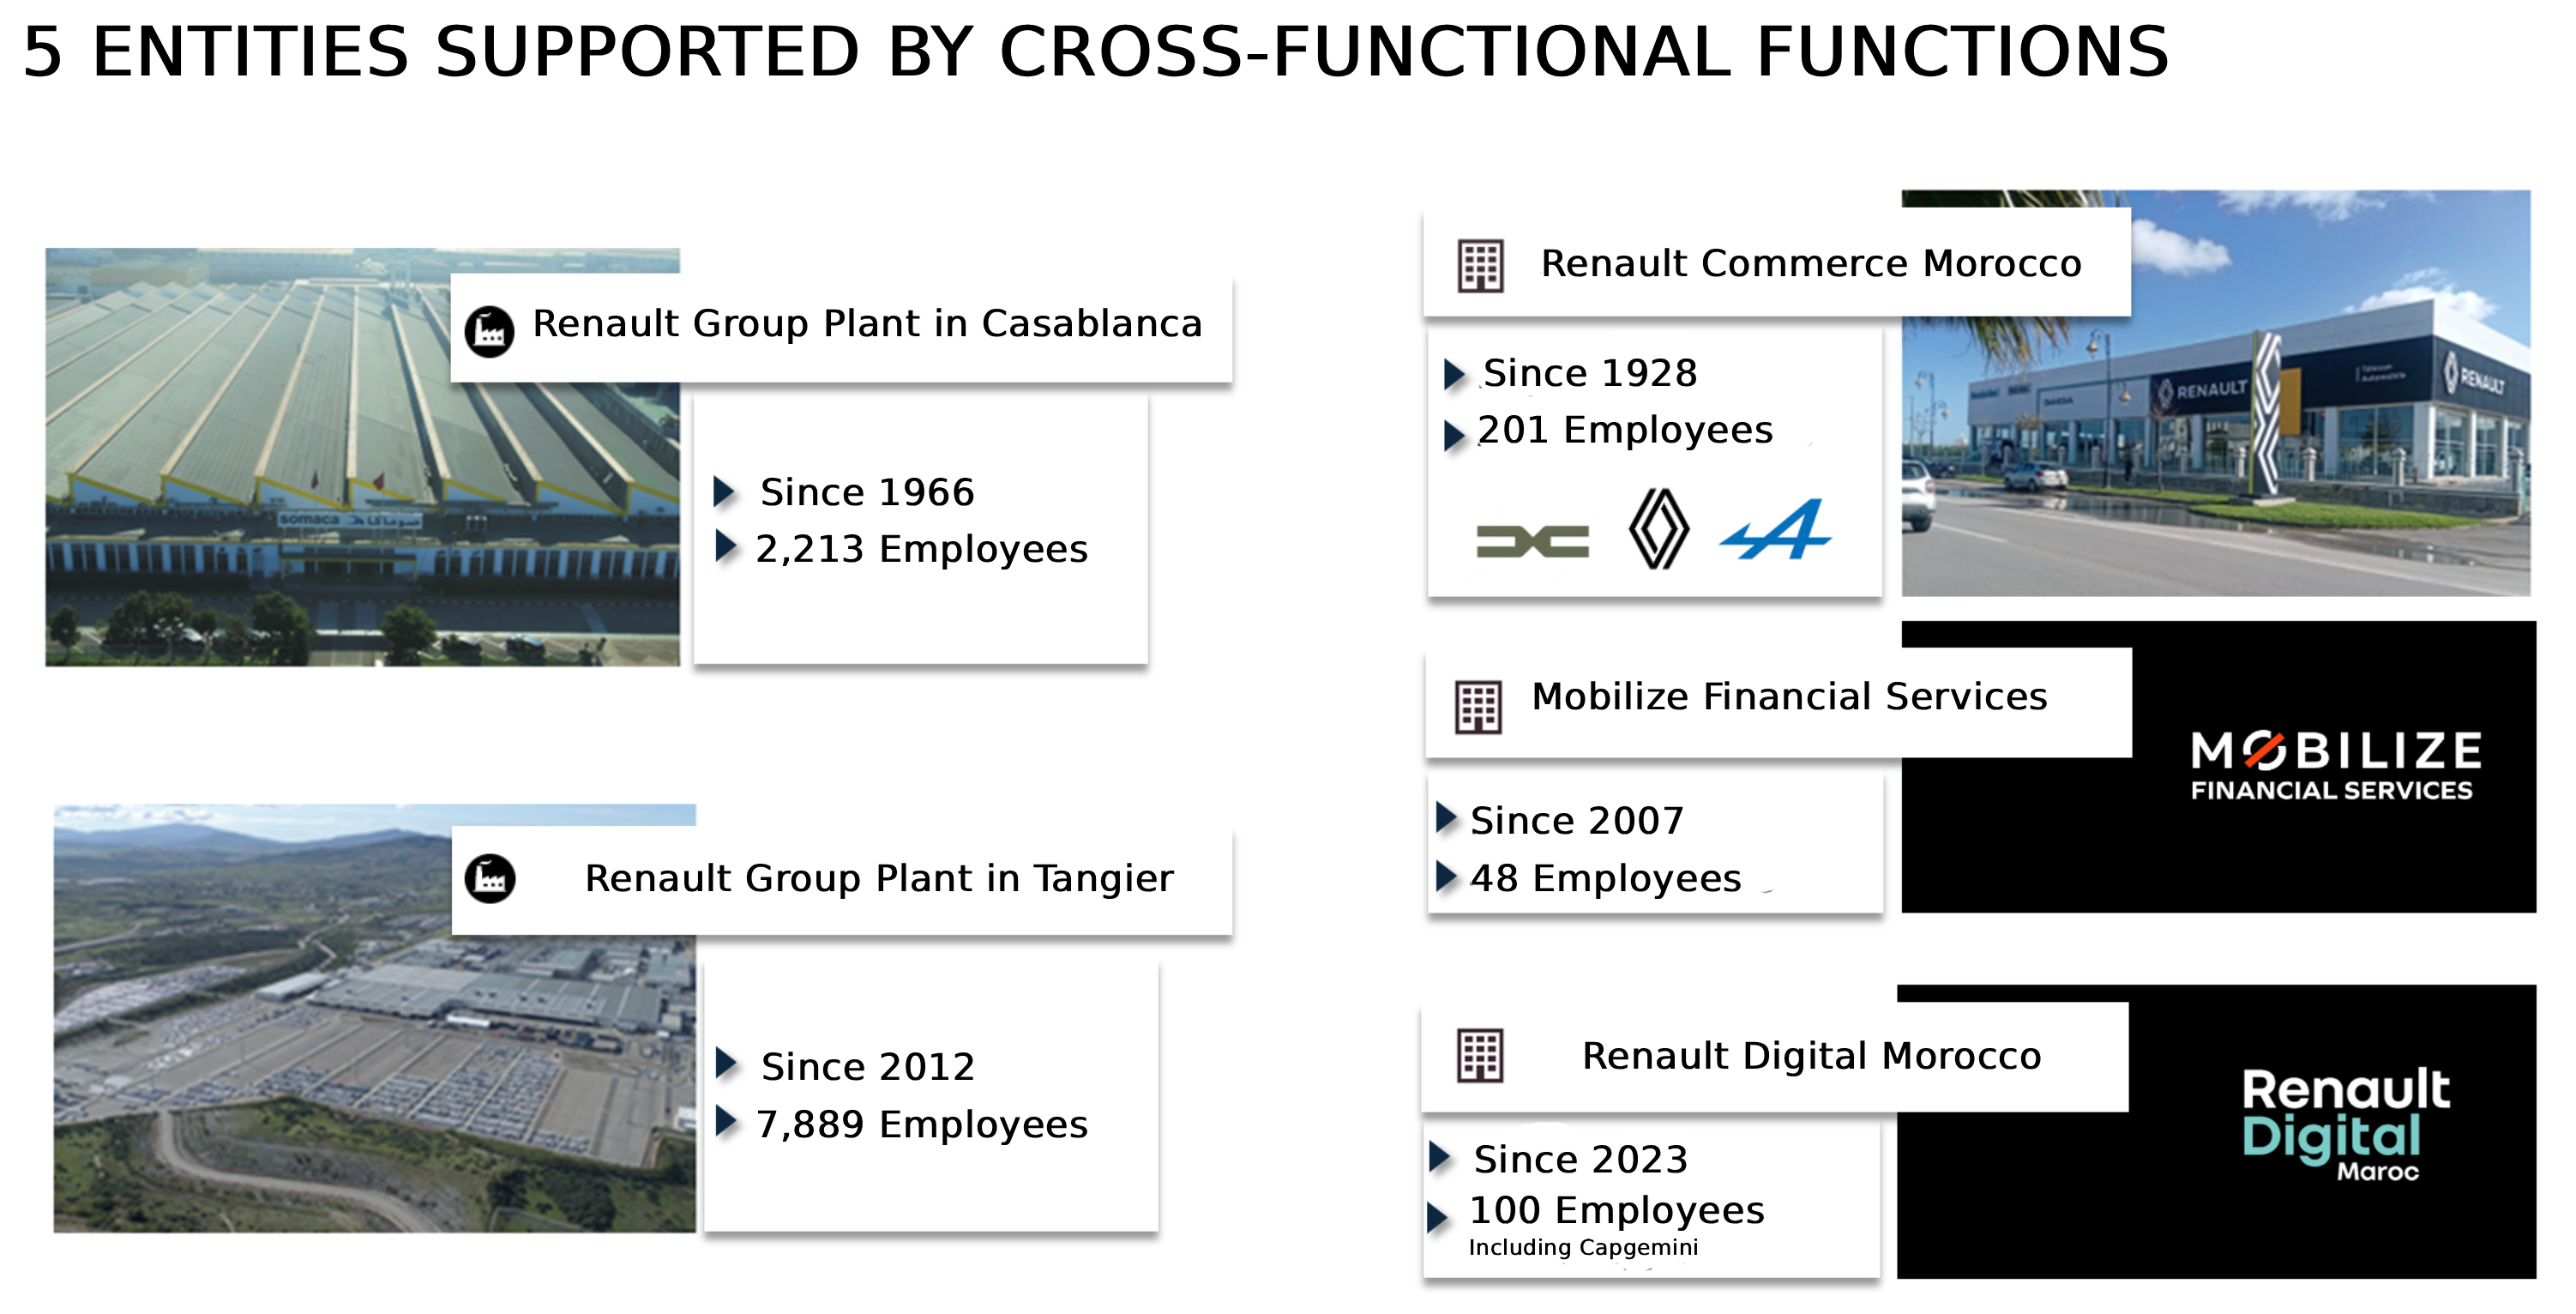
\includegraphics[width=1\linewidth]{images/renault's_entities.png}
    \caption{Entities of Renault Group Morocco}
\end{figure}

\subsection{Renault Digital Morocco}
\textbf{Renault Digital Morocco} (also called RDM) is a subsidiary of the Renault Group that supports the group in its digital transformation. RDM focuses on the development and maintenance of digital projects for all business sectors of the company and its suppliers worldwide, covering areas ranging from design and manufacturing to marketing and after-sales.



\section{Project presentation}

\subsection{General project context}
In a context where cybersecurity is becoming a major issue for the automotive sector, the Renault Group has undertaken the development of a centralized cryptographic key management system, called \textbf{Key Management System (KMS)}. This project is part of a desire to strengthen the company's security posture, while ensuring compliance with international standards and regulatory requirements of the sector.

\noindent
The \textbf{KMS} has the main objective of centrally managing all cryptographic keys used within the Renault Group, by offering:
\begin{itemize}
    \item Compliance with international regulations and cryptographic key management best practices.
    \item Enhanced security of vehicles through the management of the lifecycle of cryptographic objects.
    \item Implementation of new automated uses such as key exchange, their diversification by vehicle, or inventory management.
\end{itemize}

\noindent
The system consists of several complementary modules:
\begin{itemize}
    \item \textbf{KMS Client Module}: a REST API that securely exposes cryptographic operations to internal applications and suppliers;
    \item \textbf{CipherTrust Appliances}: hardware equipment ensuring secure storage and cryptographic operations;
    \item \textbf{KMS Web Portal}: a web interface allowing key management, access rights management, as well as inventory visualization;
    \item \textbf{KMS Admin Module}: intermediate module between the web portal and cryptographic equipment, ensuring notably signature requests to the PKI.
\end{itemize}

\newpage
\section{Project management}

\subsection{Agile development method}
Agile development is an iterative and incremental approach for project management and software development. The development team delivers iteratively and incrementally based on the priority of user needs. In agile development, a project is divided into several sub-projects before development. Each sub-project is tested and integrated, and it must also be visible and usable before delivery.\\

\noindent
Agile development allows the development team to continuously deliver products, reduce risks, constantly improve the quality of team development, be flexible to changes in user needs and improve customer satisfaction in an iterative development process.

\subsection{Scrum development}
Scrum is an agile development framework and an incremental and iterative development process. The Scrum team consists of a development team, the Scrum Master and the Product Owner (PO).\\

\noindent
With the agile development method, all client needs are considered as User Stories (US). They are provided by the PO. All US are listed in the Product Backlog with its priority given by PO. The development team delivers incrementally and iteratively products according to the Product Backlog. Agile development divides the project duration into Sprints. Before development, the development team and the PO determine the Sprint cycle. The development team estimates its velocity. After each Sprint Planning, the development team chooses User Stories for this Sprint based on its velocity and the priority of User Stories. The development team delivers the products developed in this Sprint after each Sprint, and reviews this Sprint to improve the development quality of the next Sprint.

\subsection{Scrum Board}

The \textit{Scrum Board} is a visual board that represents the progress of tasks during a sprint. 
It is divided into several columns representing the different states of a task, from its planning to its completion. 
Each task is materialized by a ticket that moves from left to right as it progresses.  

\noindent
A typical example of a Scrum Board includes the following columns: 
\textbf{To Do}, 
\textbf{In Progress}, 
\textbf{Blocked}, 
\textbf{Testing/Review} and 
\textbf{Done}. 
This system provides immediate visibility on the sprint's progress, facilitates coordination between team members and helps quickly identify potential blocking points.  

\begin{figure}[H]
    \centering
    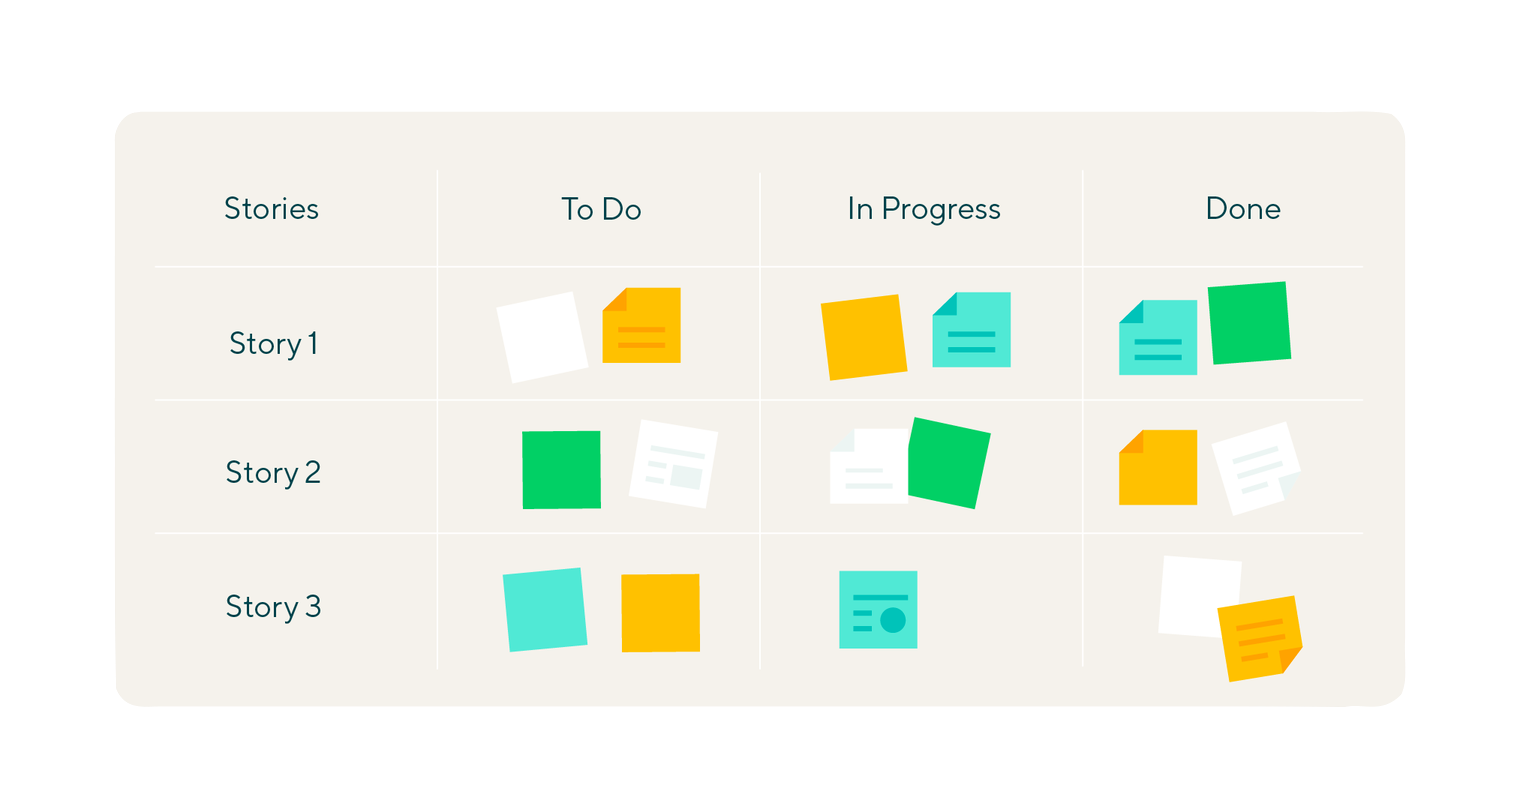
\includegraphics[width=0.8\textwidth]{images/scrum_board.png}
    \caption{Example of Scrum Board structure}
\end{figure}

In the context of this project, the \textbf{Jira} tool was used to implement the Scrum Board. 
Jira is an agile project management platform widely adopted in the industry. 
It not only allows managing tasks in the form of tickets, but also configuring \textit{workflows} adapted to the team, tracking progress via indicators (such as \textit{burndown charts}) and centralizing communication around the project.  

\begin{figure}[H]
    \centering
    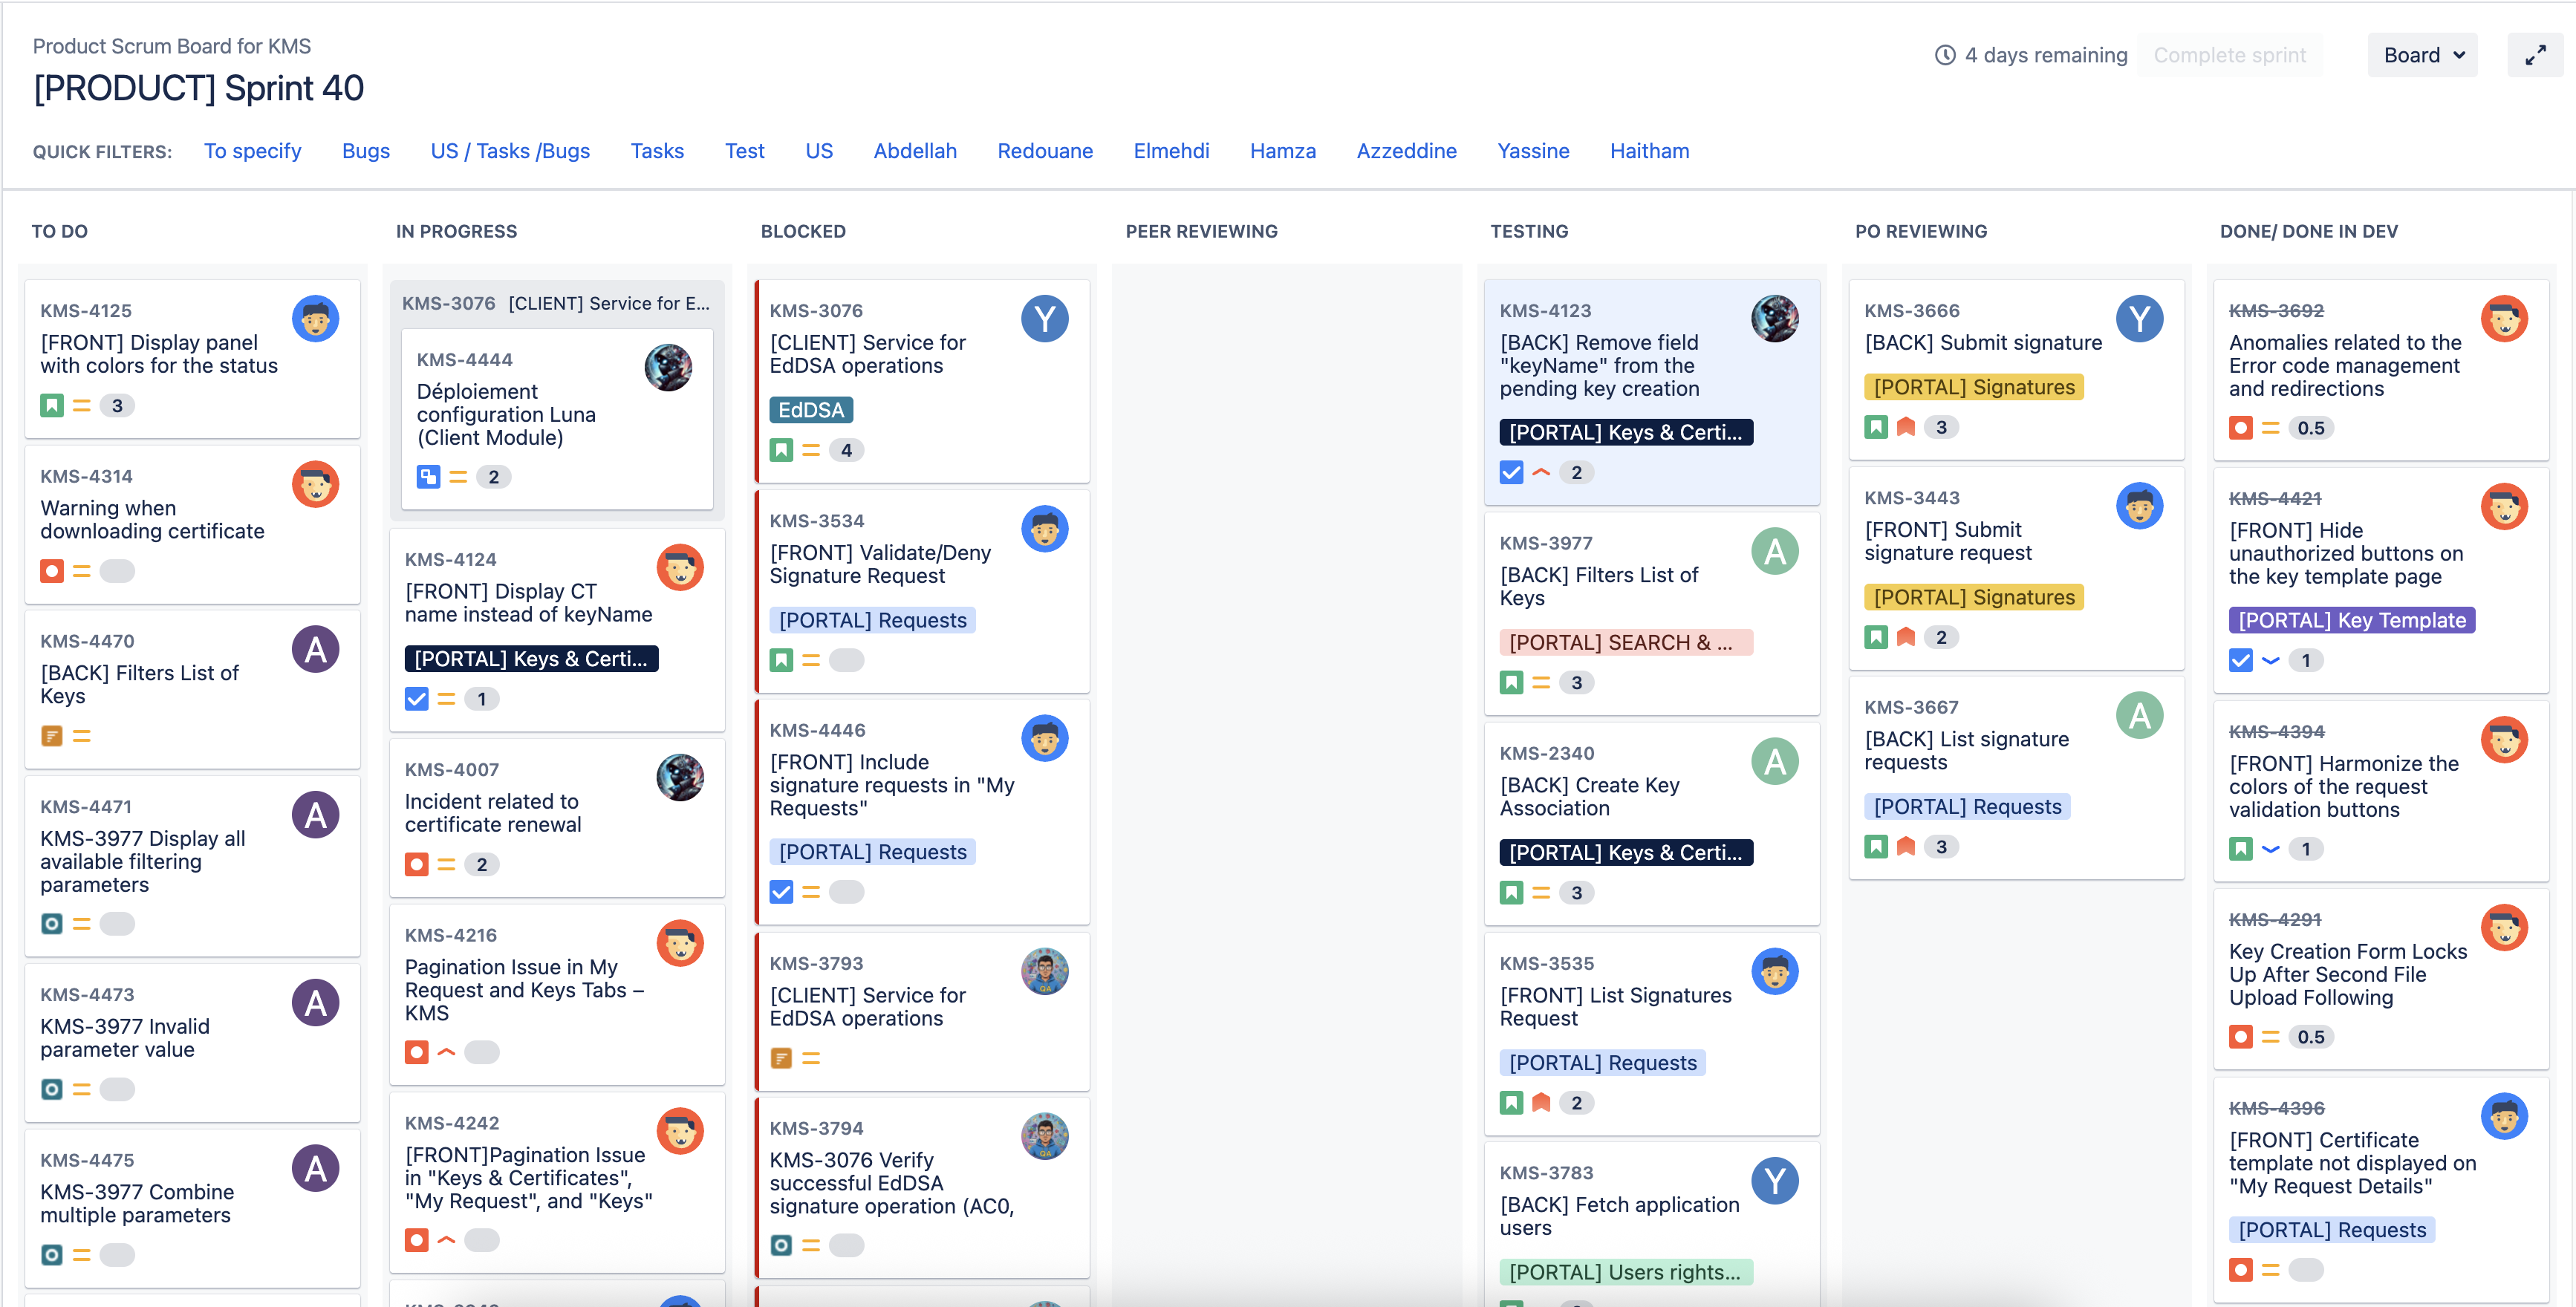
\includegraphics[width=0.9\textwidth]{images/jira_scrum_board.png}
    \caption{Real project Scrum Board under Jira}
\end{figure}

\subsection{Scrum Ceremonies}

Scrum ceremonies are regular meetings that structure the work rhythm and ensure effective communication within the team. In the context of this project, five main ceremonies were implemented:

\noindent
\textbf{Daily Meeting (Daily Standup):} A short daily meeting of 15 minutes maximum where each team member shares what they accomplished the previous day, what they plan to do today, and any obstacles they encounter. This ceremony ensures daily synchronization and rapid identification of blocking points.

\noindent
\textbf{Backlog Refinement:} Regular sessions where the Product Owner and the development team review, estimate, and prioritize User Stories in the Product Backlog. These meetings help clarify requirements, break down complex stories, and ensure that the backlog remains up-to-date and ready for future sprints.

\noindent
\textbf{Sprint Review:} A meeting held at the end of each sprint where the development team demonstrates the completed functionalities to stakeholders. This ceremony allows for immediate feedback collection and validation that the developed features meet expectations.

\newpage
\noindent
\textbf{Sprint Retrospective:} A reflection meeting where the team analyzes what went well, what could be improved, and defines concrete actions for the next sprint. This ceremony promotes continuous improvement of working methods and team dynamics.

\noindent
\textbf{Sprint Planning:} A meeting at the beginning of each sprint where the team selects User Stories from the Product Backlog and defines the sprint objective. The team estimates the effort required and commits to delivering specific functionalities within the sprint timeframe.

\section{Problematic and Objectives}

\subsection{Problem Statement}

As part of the ongoing development of the Key Management System (KMS) at Renault Group, a critical requirement has emerged for proactive management of cryptographic resource lifecycles. The KMS is being designed to centrally manage certificates, keys, and other cryptographic objects that are essential for vehicle security and internal applications.

\subsubsection{Identified System Requirements}

\textbf{Proactive Expiration Management:} The KMS needs to include functionality that proactively identifies and alerts stakeholders about upcoming certificate and key expirations. Without this capability, the system would only provide storage and management functions without preventing potential service disruptions.

\noindent
\textbf{Role-Based Notification Requirements:} The system design requires that notifications reach the appropriate personnel based on their roles and responsibilities within the organization. Different stakeholders have varying levels of responsibility for cryptographic resource management, and the notification system must account for these distinctions.

\noindent
\textbf{Multi-Channel Communication Needs:} Modern enterprise applications require multiple communication channels to ensure message delivery and user engagement. The KMS must support both formal notification channels (email) and real-time communication (in-app notifications) to meet diverse user preferences and operational requirements.

\subsection{Project Objectives}

\subsubsection{Primary Objectives}

\textbf{Implement Proactive Resource Monitoring:} Develop a notification system that automatically identifies certificates and keys approaching expiration and initiates appropriate alerts to responsible stakeholders.

\noindent
\textbf{Design Role-Based Notification Targeting:} Create a sophisticated targeting mechanism that identifies and notifies only relevant users based on their specific roles and their association with particular applications and resources.

\noindent
\textbf{Establish Multi-Channel Communication:} Implement both email and real-time in-app notification channels to ensure reliable message delivery and accommodate different user preferences and operational contexts.

\subsubsection{Secondary Objectives}

\textbf{Implement Strategic Notification Timing:} Develop a notification schedule that provides early warnings while escalating urgency as expiration approaches, balancing user awareness with notification fatigue.

\noindent
\textbf{Provide Operational Flexibility:} Include feature flag controls that allow runtime configuration of notification channels, supporting testing scenarios and phased deployment strategies.

\noindent
\textbf{Maintain Comprehensive Audit Trails:} Implement notification history tracking for compliance reporting and system monitoring, documenting when notifications were sent, to whom, and their delivery status.

\newpage
\subsection{Project Planning (Gantt Diagram)}

Our project is managed following a chronological breakdown into phases, which specifies what needs to be done (the tasks) and by whom (the resources). To represent this distribution, we use a Gantt diagram, a type of bar chart that illustrates a series of tasks over a given period. This diagram displays the list of activities to be carried out in the project, as well as their start and end dates, and constitutes a visual representation of a project schedule.

Here is an example of our Gantt diagram:

\begin{figure}[H]
    \centering
    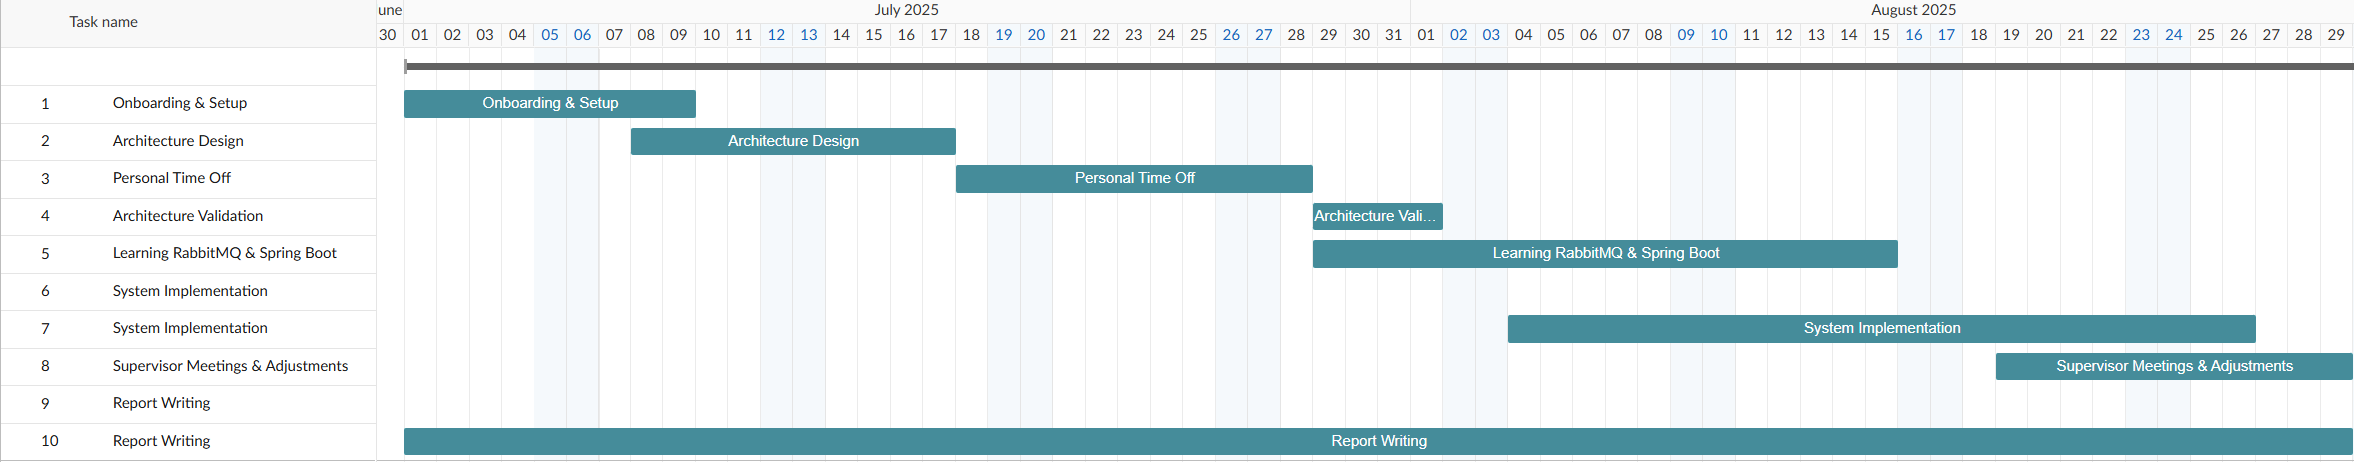
\includegraphics[width=1\linewidth]{images/gantt_diagram.png}
    \caption{Project Planning Gantt Diagram - July 1 to August 31}
    \label{fig:gantt_diagram}
\end{figure}

\section*{Conclusion}

This chapter established the foundation for understanding the project context within Renault Group's digital transformation initiative. The presentation of the KMS project highlighted the critical need for automated management of cryptographic resource lifecycles, particularly the challenge of proactive expiration monitoring and notification. The adoption of Agile methodology with Scrum framework, supported by appropriate project management tools, provides a structured approach for delivering this complex notification system that will enhance the security posture of Renault's cryptographic infrastructure.